\section{DnsPacket}\label{sec:dnspkt}

\begin{figure}
\begin{center}
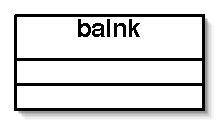
\includegraphics[width=0.4\textwidth]{figs/blank}
\end{center}
\caption{}
\label{fig:dnspkt}
\end{figure}

This section describes the component, which is described by Figure~\ref{fig:dnspkt}.  

This component represents a high-level view of a DNS packet. It encapsulates all the header information as well as the RRs that were received from the wire.


\subsection{Methods}

{\bf Public Methods}
\begin{itemize}
\item add\_bytes(): This method is called by the resolver when bytes have been received from the network. It can be called as many times as necessary and will continue to add bytes to the buffer. For a UDP packet, this will only be called once. However, this can be called arbitrarily many times for a TCP packet.
\item parse(): Once all the data has been received from the wire, calling this method parses the packet and returns a boolean value depending on the success or failure of the parse.
\item to\_wire(): This method converts the message from high-level objects into the canonical wire representation of a DNS packet.
\item header(): This method returns the header section of the DNS packet.
\item questions(): This method returns a list of the question RRs from the packet.
\end{itemize}

{\bf Private Methods}
\begin{itemize}
\item clear\_vectors(): This method frees the memory associated with the RRs and is used by the destructor.
\end{itemize}

\subsection{Member Variables}
\begin{itemize}
\item m\_header: A DnsHeader object representing the parsed headers.
\item m\_qd: Question RRs from the original DNS packet.
\item m\_an: Answer RRs from the original DNS packet.
\item m\_ns: Authoritative NS RRs from the original DNS packet.
\item m\_ar: Additional RRs from the original DNS packet.
\item m\_bytes: Buffer of bytes from the network.
\end{itemize}
